\vspace{-2.5cm}
\begin{tikzpicture}
    \node (park) [blurb] {
    \newline{\fontsizetitle Moltres}\\
    \vspace{-20pt}\rule{\textwidth}{5pt}\\
    \fontsizesection
    S$_N$-D method for accurate time-dependent control rod modeling in Moltres, an open-source MOOSE application for the simulation of molten salt reactors\cite{park}.\\
    \begin{center}
        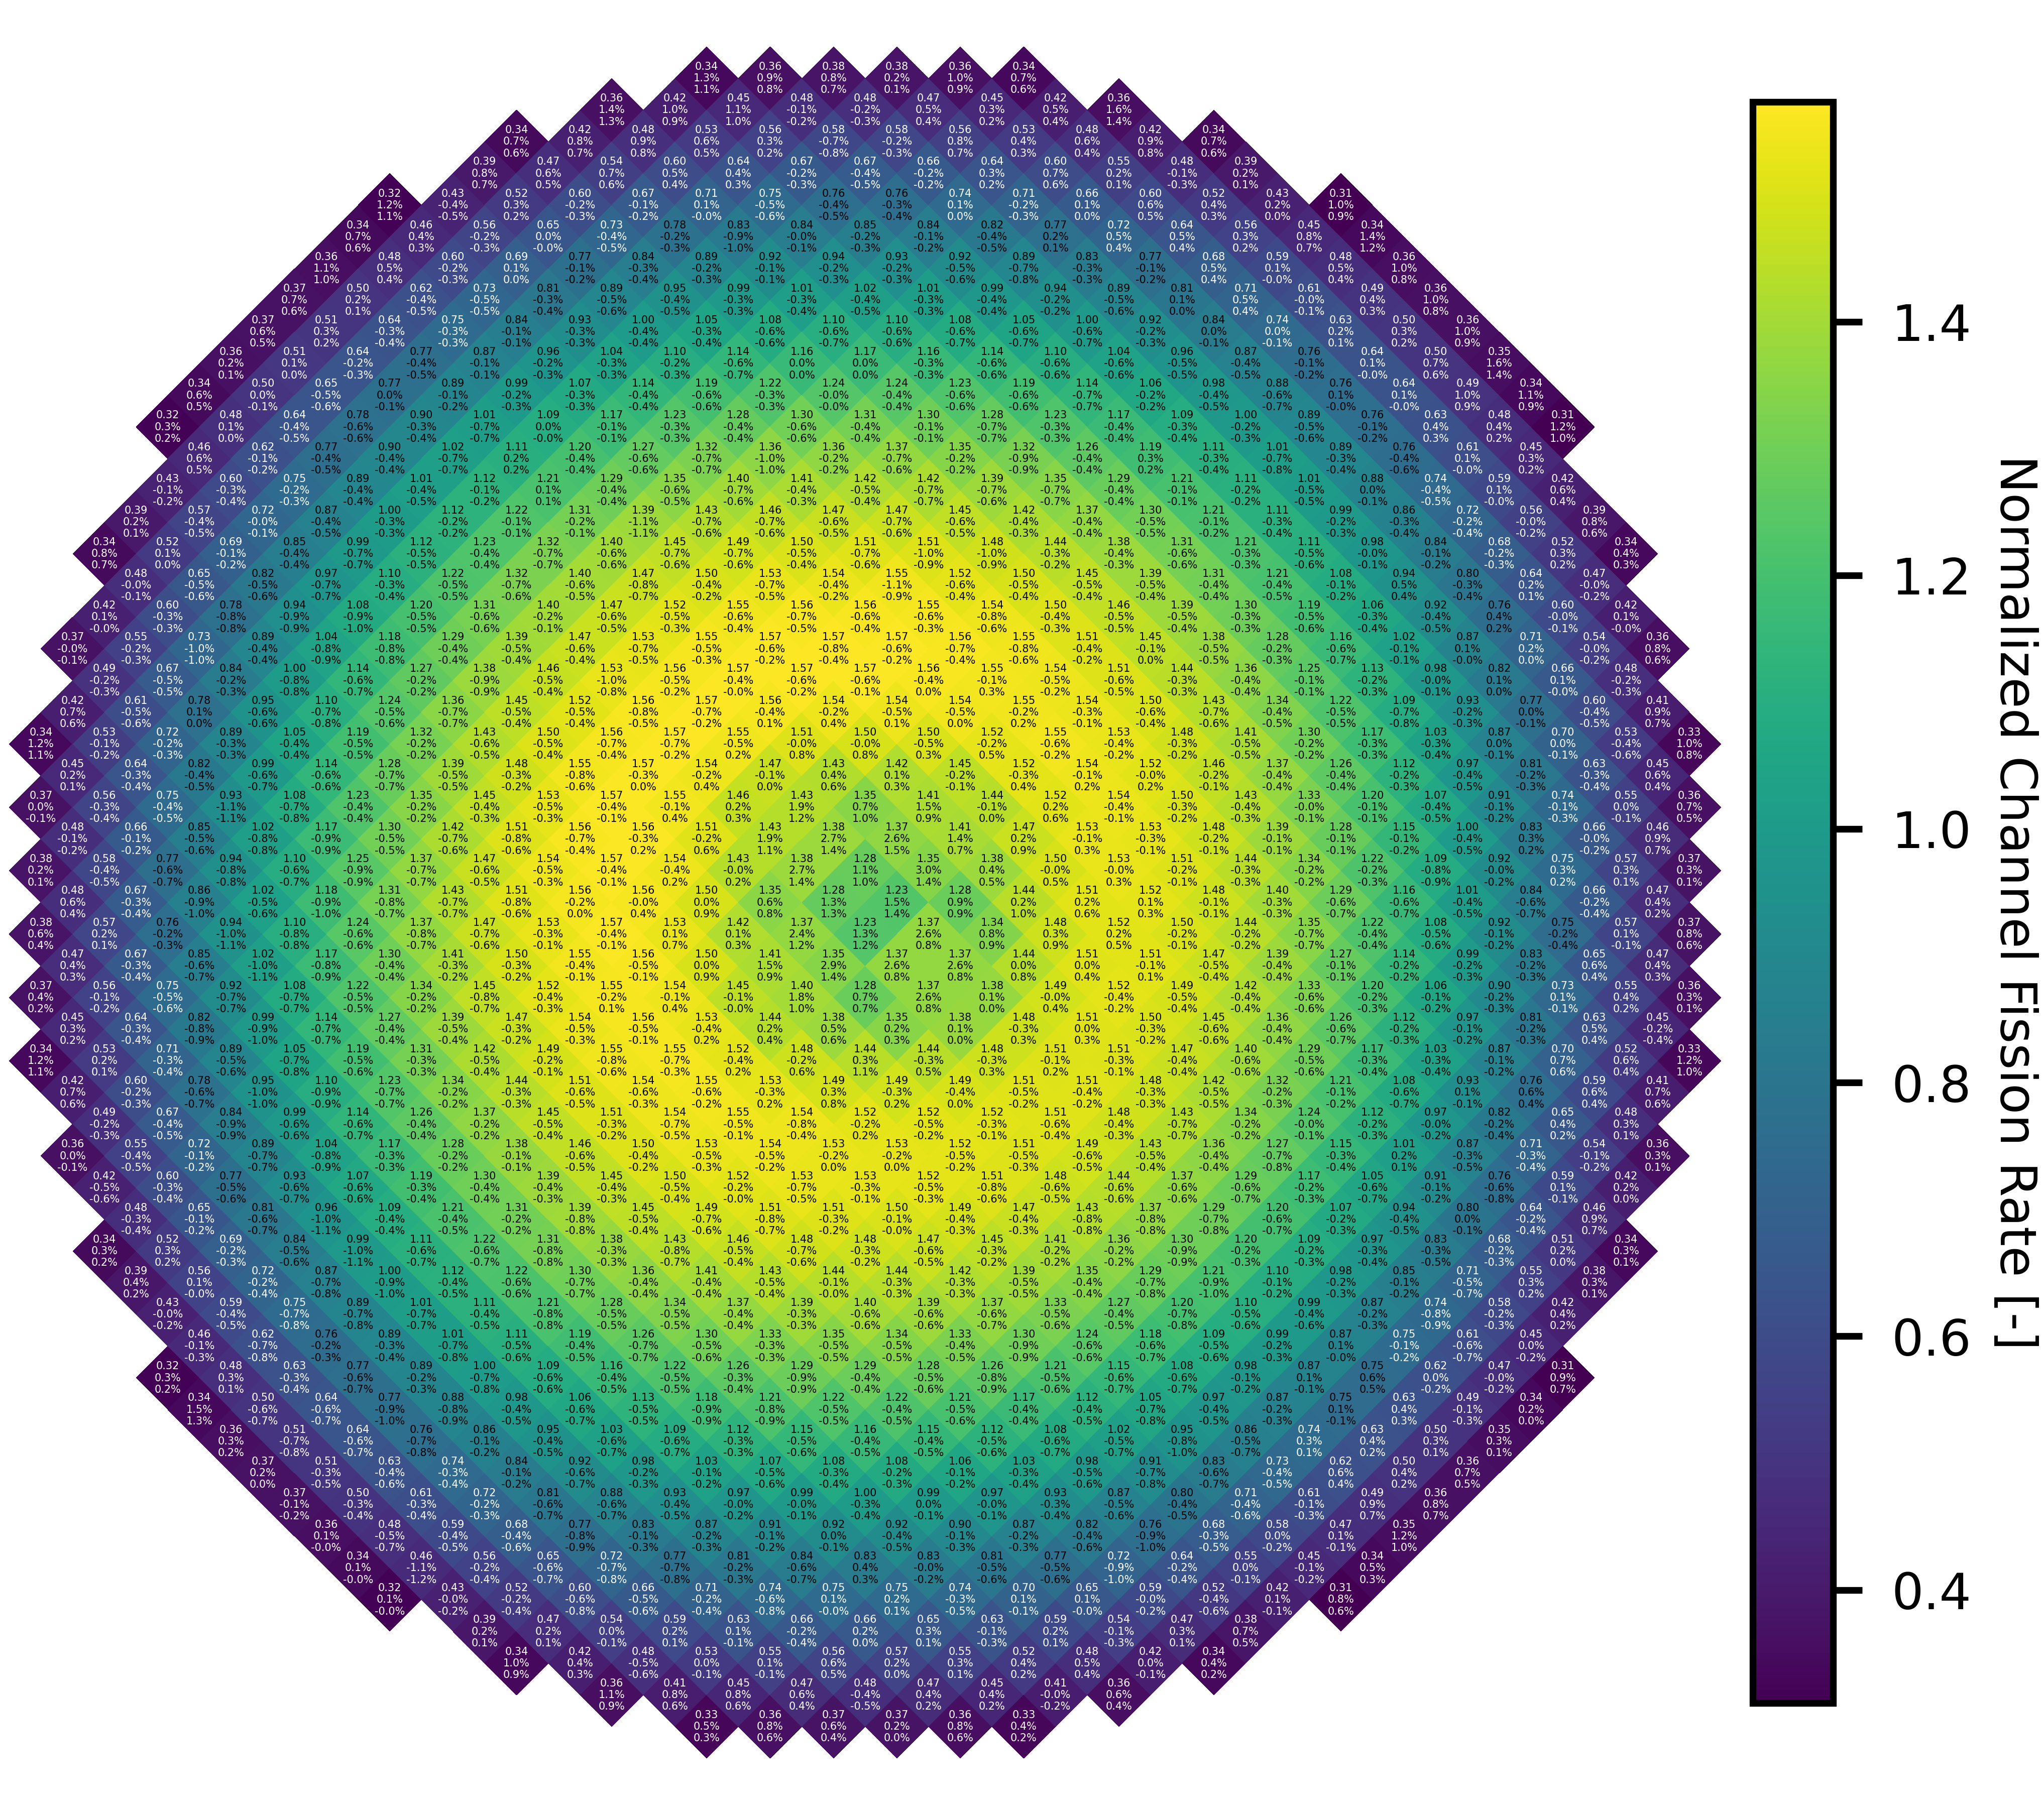
\includegraphics[width = .4\textwidth]{img/msre-full-0-power.png}
        \hspace{2cm}
        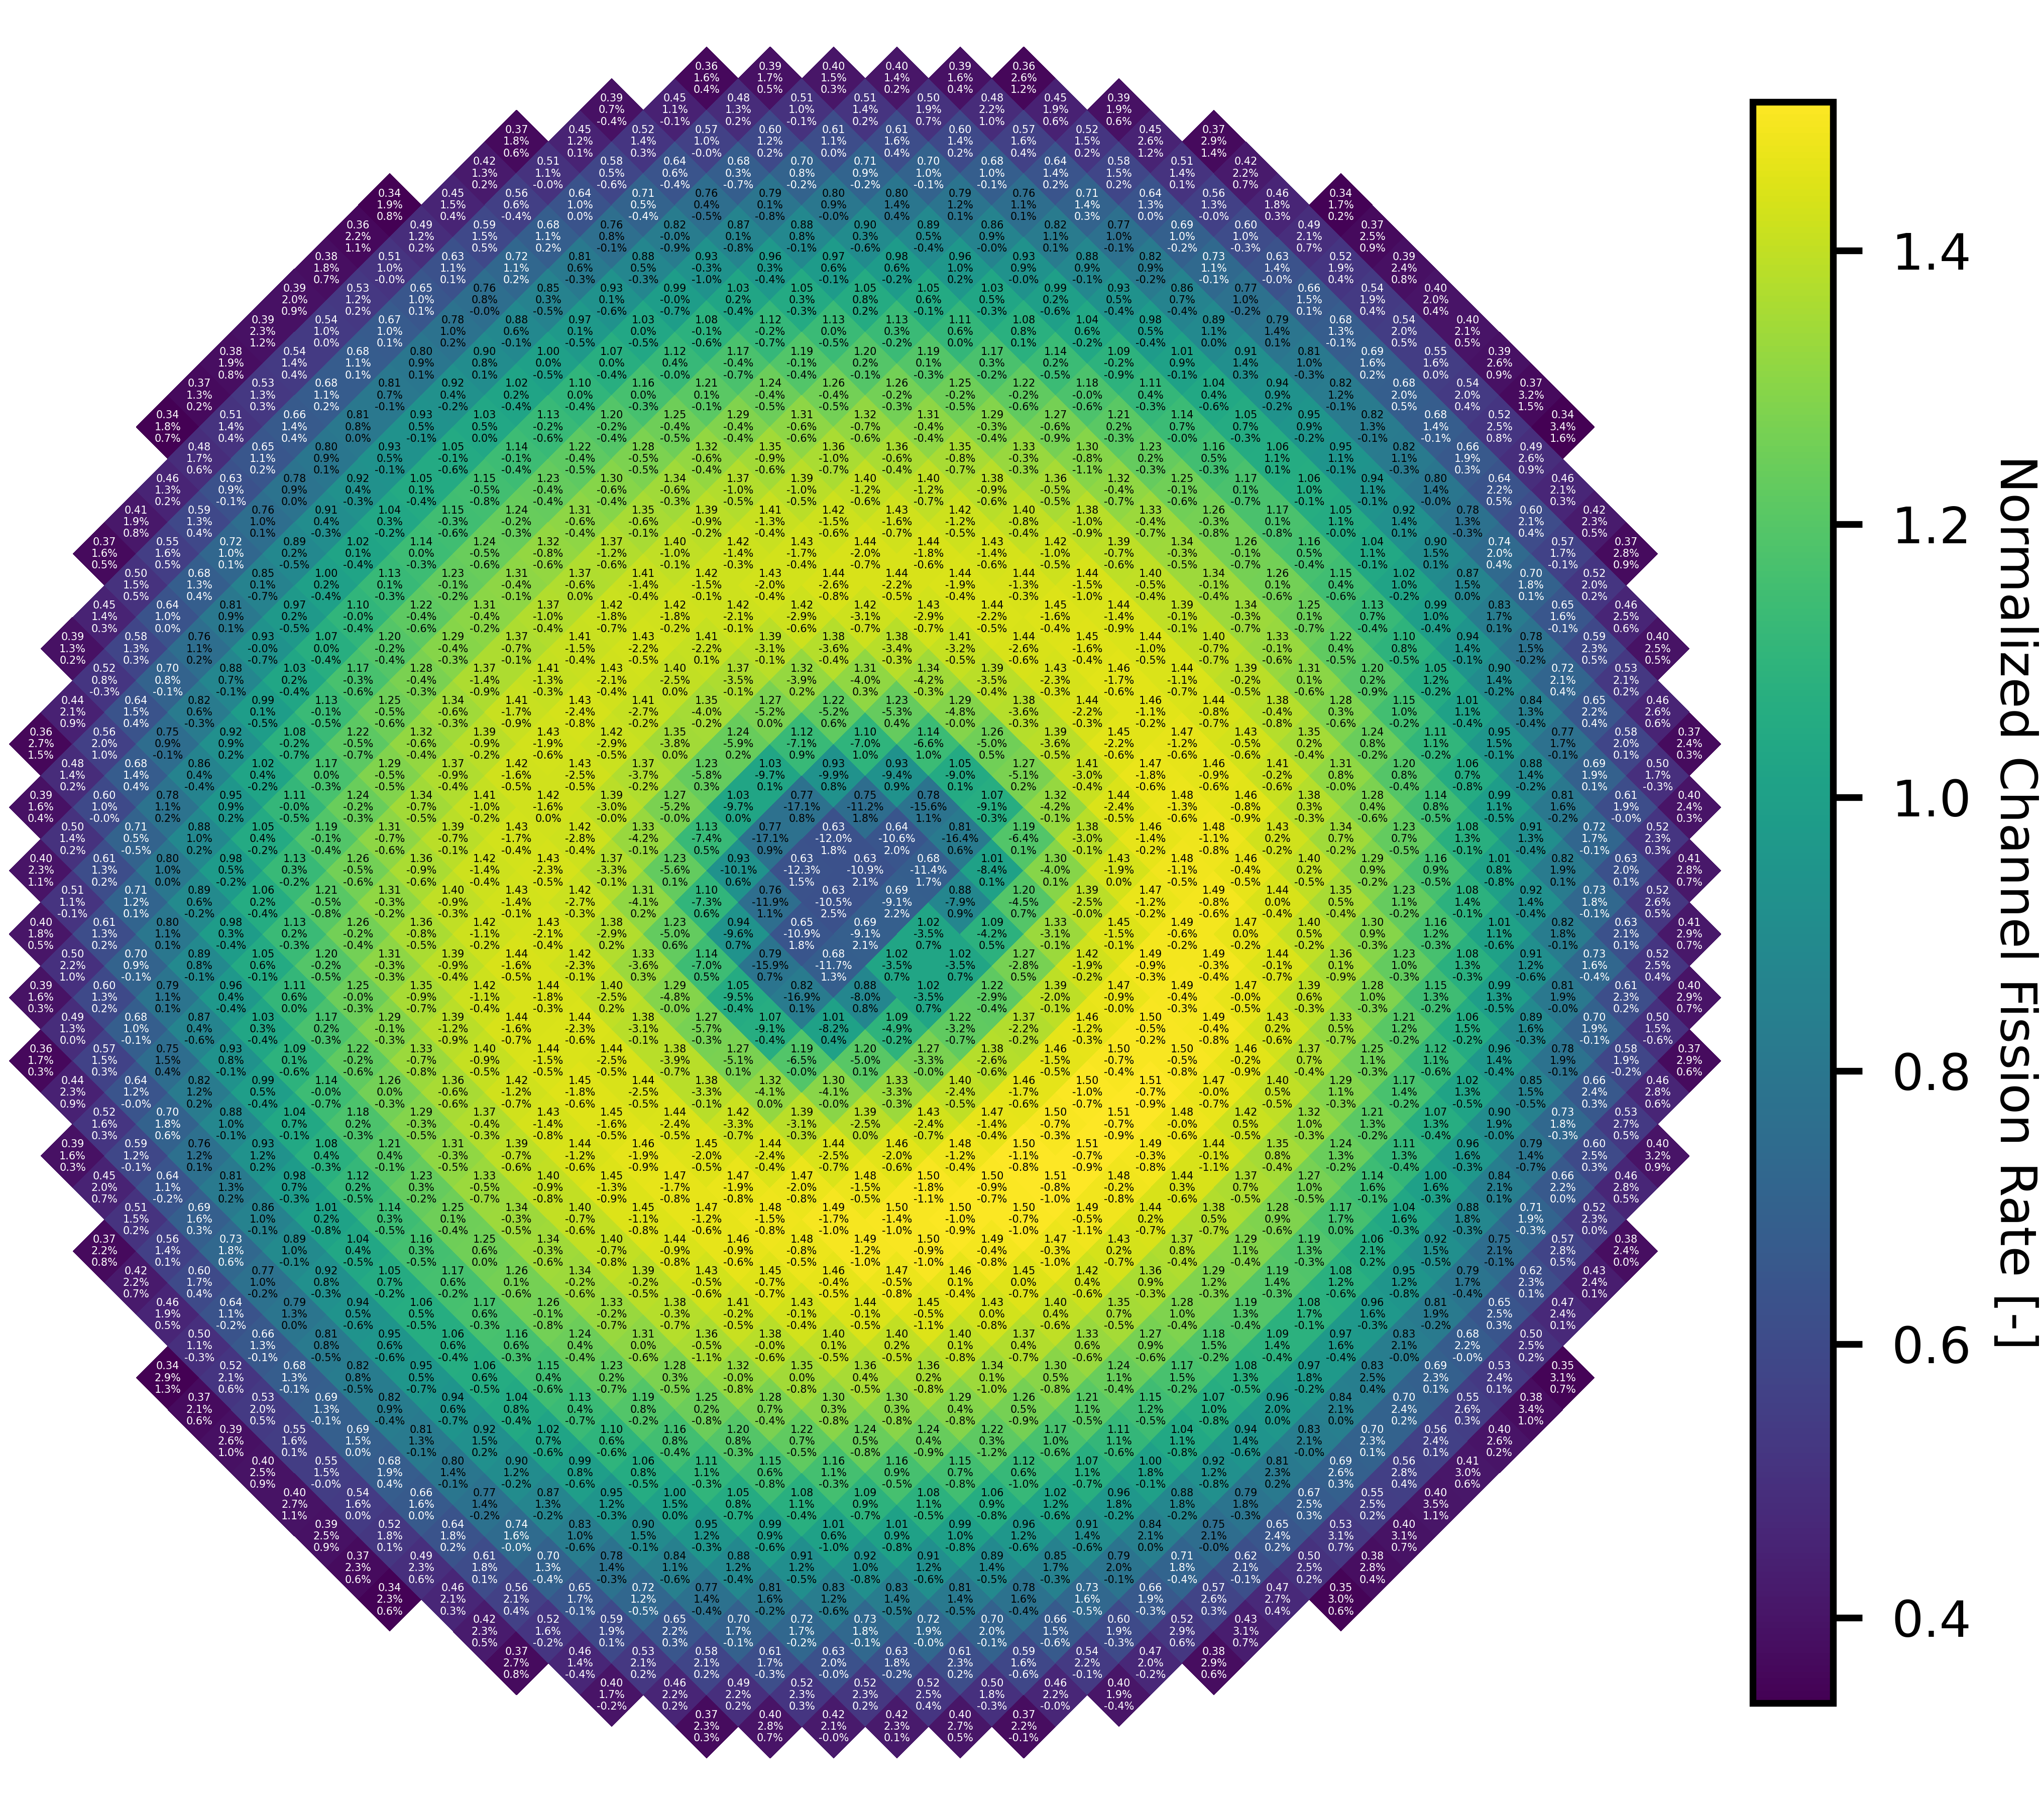
\includegraphics[width = .4\textwidth]{img/msre-full-123-power.png}
        \\
        \capt{MSRE full core scalar flux error as calculated with pure diffusion, $S_N-D$, and OpenMC for all control rods removed (left) and all control rods inserted (right)}
    \end{center}

    };
    \node (bachmann) [blurb, below of = park, yshift=-19.25cm] {
    \newline{\fontsizetitle OpenMCyclus}\\
    \vspace{-20pt}\rule{\textwidth}{5pt}\\
    \fontsizesection
    Reactor-physics informed fuel cycle analysis on the impacts of deploying HALEU-fueled reactors using OpenMCyclus, a coupling of OpenMC with Cyclus\cite{bachmann}.\\
    \begin{center}
    \begin{minipage}{.45\textwidth}
    \vspace{1cm}
        \includegraphics[width = \textwidth]{img/bachmann.jpg}\\
    
        \capt{Depletion methodology in OpenMCyclus. Blue comes from Cyclus and Red is provided through user-inputs.}
    \end{minipage}
    \hspace{1cm}
    \begin{minipage}{.45\textwidth}
    \vspace{0cm}
        \vspace{.5cm}
        \includegraphics[width = \textwidth]{img/comparison_pu_cumulative.pdf}\\
        \vspace{-1cm}
        
        \capt{Comparison of the cumulative mass of separated plutonium traded after using the OpenMCyclus and Cycamore reactor.}
    \end{minipage}
    \end{center}
    };
    \node (chee) [blurb, below of = bachmann, yshift = -20.75cm] {
    \newline{\fontsizetitle ROLLO}\\
    \vspace{-20pt}\rule{\textwidth}{5pt}\\
    \fontsizesection
    Evolutionary algorithm techniques applied to optimize nuclear reactor design by coupling nuclear software to the DEAP evolutionary algorithm driver \cite{chee}.
    \begin{center}
    \includegraphics[width = .7\textwidth]{img/assem-obj-3-2d.png}
    \\
    \capt{Triple-objective optimization to minimize total fuel packing fraction, max temp, and fuel-normalized power peaking factor in the one-third assembly}
    \end{center}
    };
\end{tikzpicture}
%% This fills the space between the content and the logo
\vfill

%% Institution logo
\begin{center}

\includegraphics[height=0.28\textwidth]{img/UIUC_Logo.png}\hspace{5cm}
\includegraphics[height=0.28\textwidth, trim={0 .5cm 0 .5cm}]{img/arfc_atom.png}

\end{center}